%%%%%%%%%%%%%%%%%%%%%%%%%%%%%%%%%%%%%%%%%%%%%%%%%%%%%%%%%%%%%%%%%%%%%%%%
% TFG: Vigilancia Tecnológica y Minería de Opiniones en RRSS
% Escuela Técnica Superior de Ingenierías Informática y de Telecomunicación
% Realizado por: Miguel Keane Cañizares
% Contacto: miguekeca@correo.ugr.es 
%%%%%%%%%%%%%%%%%%%%%%%%%%%%%%%%%%%%%%%%%%%%%%%%%%%%%%%%%%%%%%%%%%%%%%%%

\chapter{Metodología}

El proyecto constará de varias fases importantes a tener en cuenta, de las cuales distinguiremos de forma importante cuatro. Preparación, Desarrollo, Obtención de Información y Análisis de resultados. 

\subsection{Preparación}

Esta fase será tiempo dedicado principalmente al estudio del lenguaje de programación Python, estudiando sus diferentes librerías, tales como NumPy\cite{Numpy}, Pillows\cite{Pillow}, Pandas\cite{Pandas} y Matplotlib\cite{Hunter:2007}. Además de cómo aplicar los conocimientos de programación obtenidos durante el grado en este lenguaje el cual es la primera vez que utilizo. Además será necesario conocer cómo funciona la API de Twitter y la API de MeaningCloud\cite{MeaningCloud}, para poder extraer la información y luego analizarla. Repasar cómo funciona una base de datos MongoDB\cite{MongoDB}, utilizada previamente durante los años lectivos, pero en necesidad de refrescar los conocimientos. 

También ha sido elegida LaTeX\cite{goossens93} para el desarrollo de la memoria, cuyos parámetros también habrán de ser estudiados para la correcta realización del proyecto junto con las diferentes formas de creación de tablas y gráfica. 

Es importante también destacar que para el proyecto se requerirá de acceso a dos APIs distintas, por lo que es necesario registrarse en Twitter Dev (\href{https://developer.twitter.com/en/apply-for-access.html}{https://developer.twitter.com/en/apply-for-access.html})  para obtener las claves de Twitter y en la plataforma de MeaningCloud (accesible desde: \href{https://www.meaningcloud.com/developer/login}{https://www.meaningcloud.com/developer/login}), para poder hacer uso de su análisis con la clave que proporcionan.

Finalmente, se ha optado por la realización de un diagrama de Gantt para hacer un correcto seguimiento del proyecto. 

\subsection{Desarrollo}

Esta fase se dedicará al desarrollo del software correspondiente, crear los scripts que sean necesarios para obtener la información, analizarla y procesarla, almacenando la misma y sus resultados de forma correcta.

Para esto se hará un primer script, que obtendrá la información desde la API de Twitter y la almacenará en una base de datos MongoDB. 

Posteriormente será necesario otro script que tenga acceso a la información analizada en la base de datos, de la orden de analizarla con la API de MeaningCloud y almacene estos resultados en un formato para su posterior uso, como puede ser CSV. 

Además haremos otros scripts para analizar la información obtenida, usar algoritmos para crear imágenes y WordClouds.  

\subsection{Obtención de información}

Una vez desarrollados los primeros scripts, haré uso de los métodos de la API de stream para escuchar en directo con la palabra o palabras claves deseadas. Este proceso podrá ser largo y controlado, para obtener una cantidad de información aceptable para el análisis y almacenar la misma en su respectiva base de datos MongoDB. 

\subsection{Análisis de resultados}

Cuando ya disponemos de la información deseada, desde la propia base de datos MongoDB enviaremos la información a la API de MeaningCloud. La cual será procesada y la respuesta será almacenada doblemente, en una base de datos MongoDB por si requerimos de analizarla de nuevo y en un fichero CSV, el cual es ideal para luego poder estudiar los resultados. Además en esta fase se desarrollará un script que pueda crear nubes con las palabras más utilizadas en la información descargada. También se tratará de obtener conclusiones sobre los datos obtenidos que puedan ser prácticas para una empresa. 
Es importante destacar que en la versión gratuita de MeaningCloud solo tendremos 20000 créditos para gastar. Por cada tweet, debido a su longitud se gastará un crédito, por lo que no se deberán malgastar éstos, aunque probablemente sea posible obtener otra clave extra. 




%	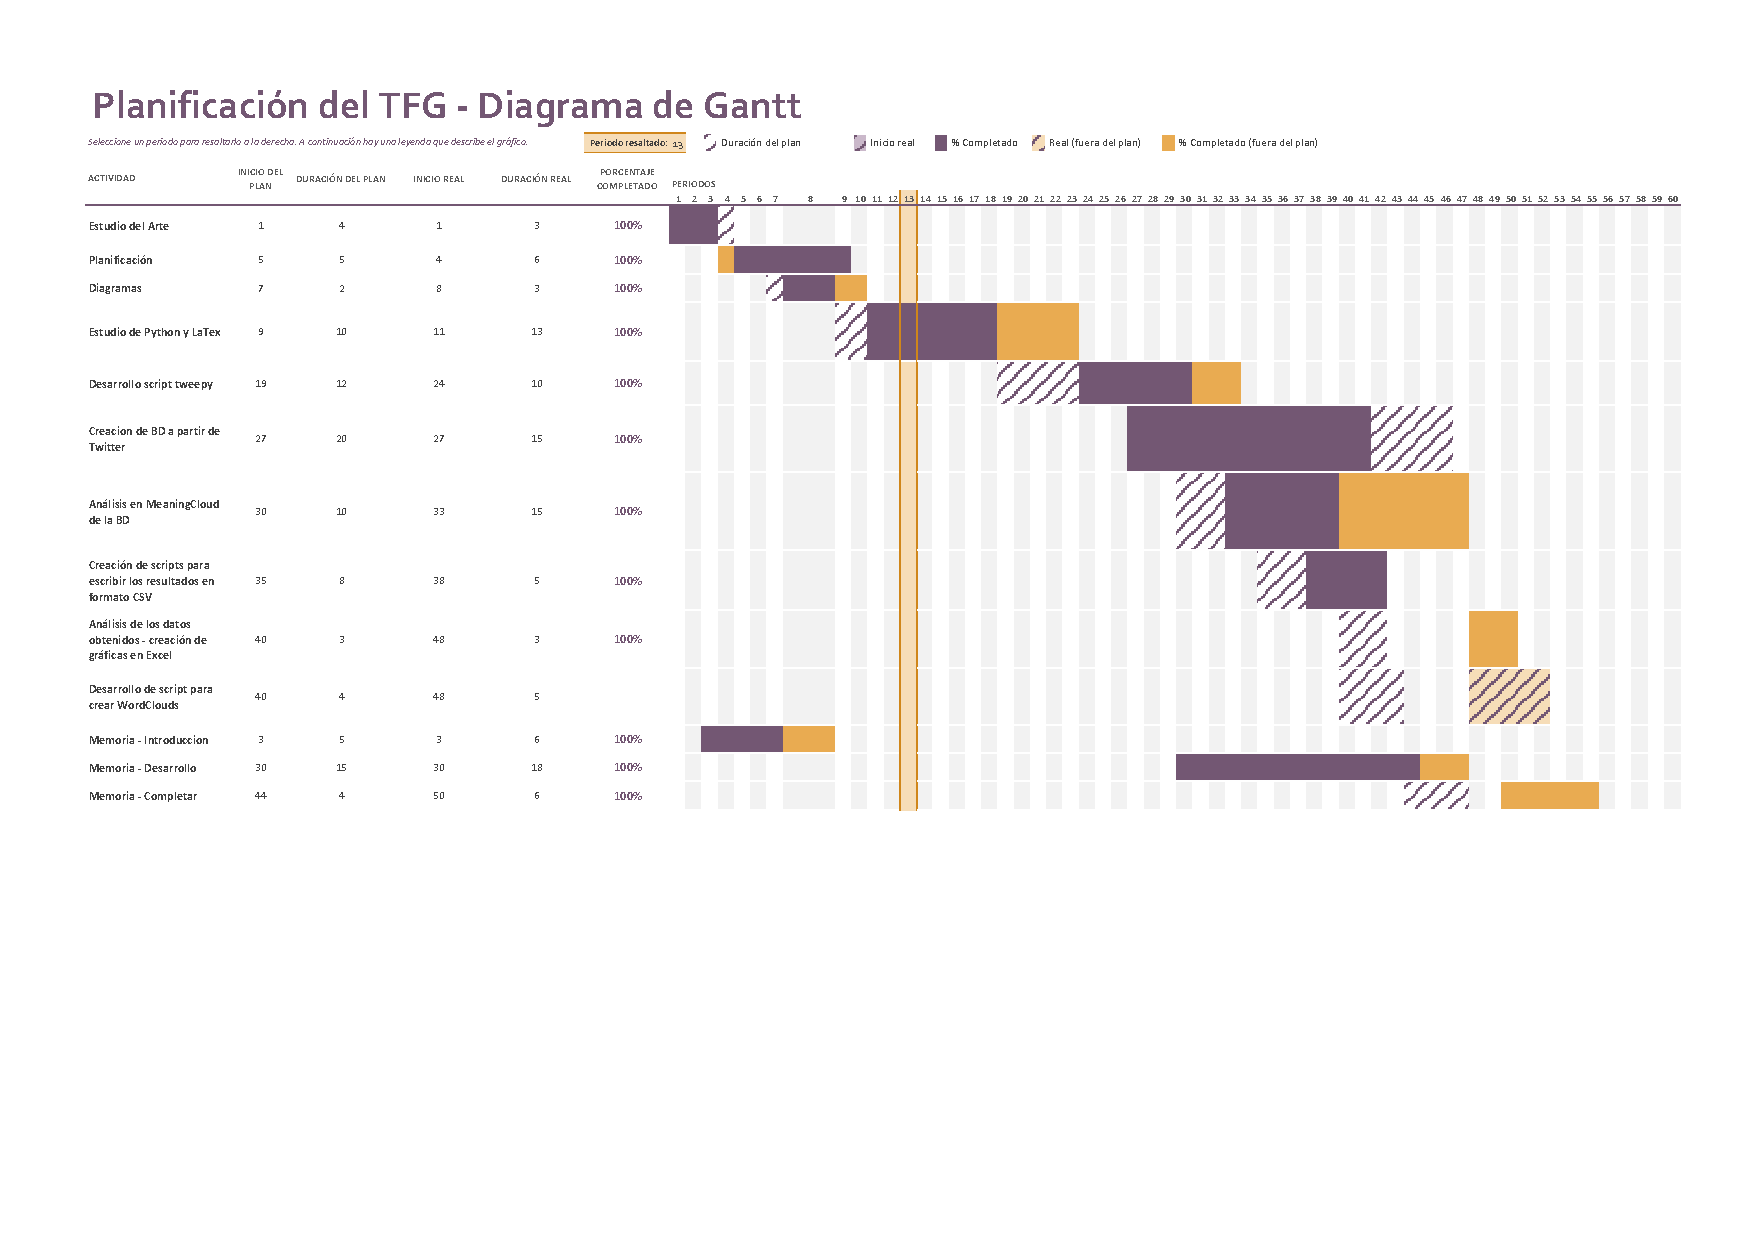
\includepdf[pages={1}]{capitulos/Gantt1-wordcloud.pdf}
En el siguiente diagrama de Gantt aparece la división de trabajo dividido entre la planificación estimada y el tiempo real de realización. Los números que aparecen en la parte superior son las horas de trabajo. Se le estimaron 48 horas en total, teniendo en cuenta que había partes del proceso que podían realizarse simultáneamente. (Mientras se descargan tweets se puede trabajar en otro script que será necesario después). Pero el resultado real, como viene destacado, fue de 56 horas de trabajo. El resto de elementos de la tabla se encuentran en la leyenda del diagrama. 

\begin{figure}[H]
	\centering
	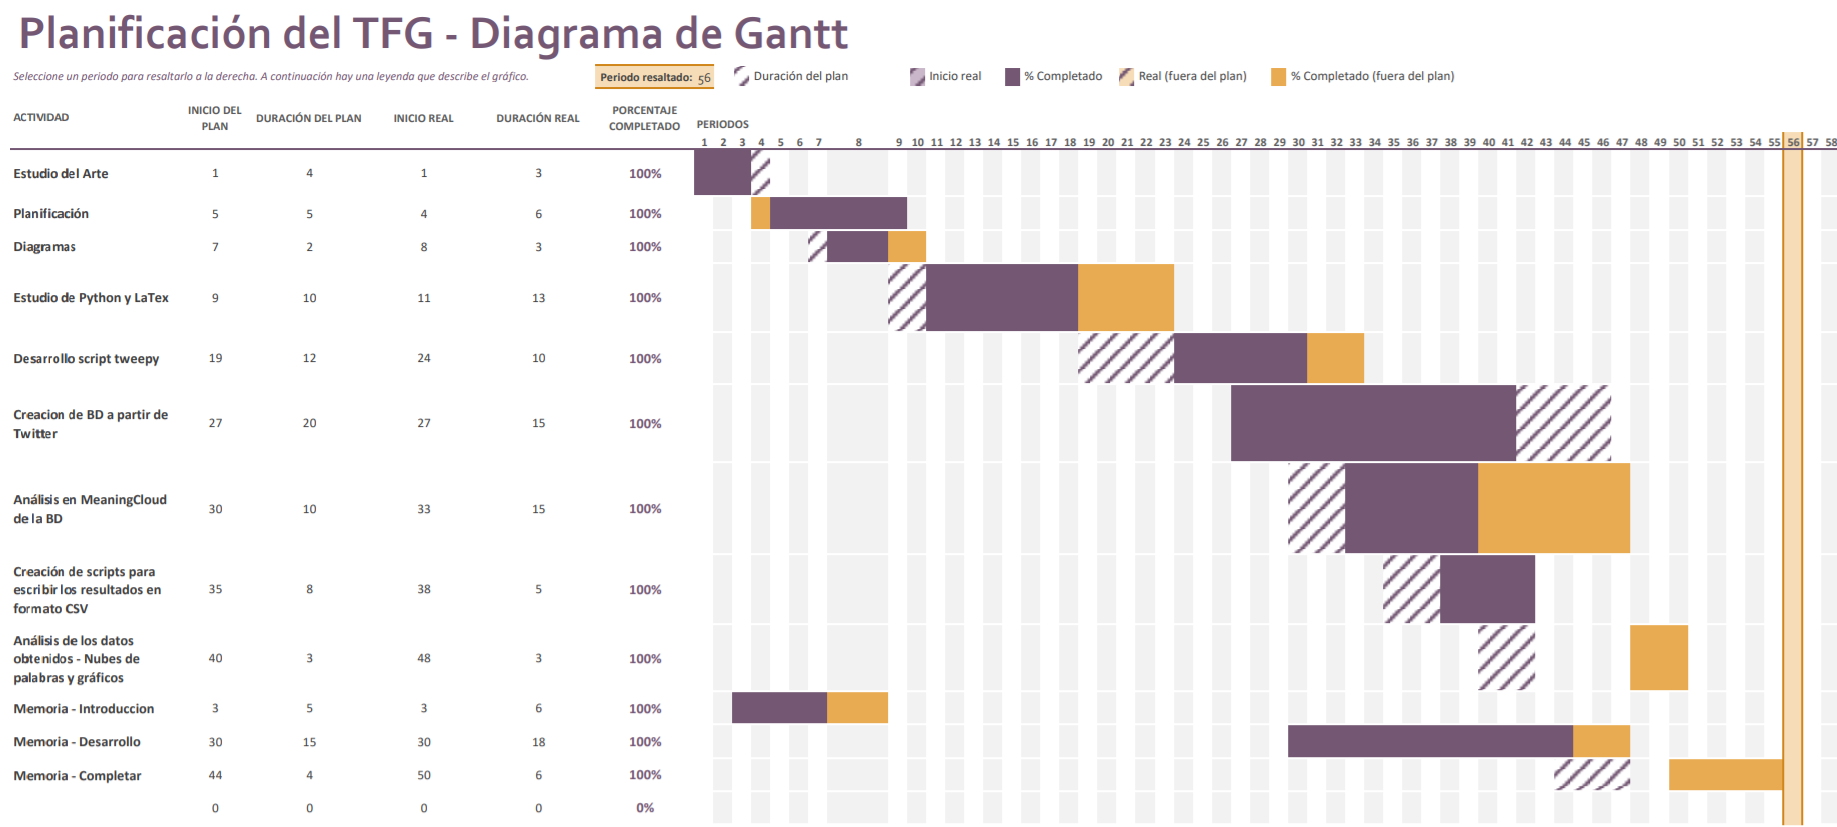
\includegraphics[scale=.45]{imagenes/ganttzoom.png}
	\caption{Diagrama de Gantt}
	\label{fig:gantt}
\end{figure}
















